%%%%%%%%%%%%%%%%%%%%%%%%%%%%%%%%%%%%%%%%%%%%%%%%%%%%%%%%%%%%%%%%%%%%%%%%%
%  Zawartość: Główny plik szablonu pracy dyplomowej (magisterskiej/inżynierskiej).
%  Opracował: Tomasz Kubik <tomasz.kubik@pwr.edu.pl>
%  Data: kwiecień 2016
%  Wersja: 0.2
%%%%%%%%%%%%%%%%%%%%%%%%%%%%%%%%%%%%%%%%%%%%%%%%%%%%%%%%%%%%%%%%%%%%%%%%%

\documentclass[a4paper,onecolumn,oneside,12pt,extrafontsizes]{memoir}
% W celu przygotowania wydruku do archiwum należy przesłonić komendę powyższą
% dwoma poniższymi komendami:
%\documentclass[a4paper,onecolumn,twoside,10pt]{memoir} 
%\renewcommand{\normalsize}{\fontsize{8pt}{10pt}\selectfont}

%\usepackage[cp1250]{inputenc} % jeśli kodowanie edytowanych plików to cp1250 
\usepackage[utf8]{inputenc} % jeśli kodowanie edytowanych plików to UTF8
\usepackage[T1]{fontenc}
%\DisemulatePackage{setspace}
\usepackage{setspace}
\usepackage{tabularx}
\usepackage{color,calc}
%\usepackage{soul} % pakiet z komendami do podkreślania tekstu

\usepackage{ebgaramond} % pakiet z czcionkami garamond, potrzebny tylko do strony tytułowej, musi wystąpić przed pakietem tgtermes

%% Aby uzyskać polskie literki w pdfie (a nie zlepki) korzystamy z pakietu czcionek tgterms. 
%% W pakiecie tym są zdefiniowane klony czcionek Times o kształtach: normalny, pogrubiony, italic, italic pogrubiony.
%% W pakiecie tym brakuje czcionki o kształcie: slanted (podobny do italic). 
%% Jeśli w dokumencie gdzieś zostanie zastosowana czcionka slanted (np. po użyciu komendy \textsl{}), to
%% latex dokona podstawienia na czcionkę standardową i zgłosi to w ostrzeżeniu (warningu).
%% Ponadto tgtermes to czcionka do tekstu. Wszelkie matematyczne wzory będą sformatowane domyślną czcionką do wzorów.
%% Jeśli wzory mają być sformatowane z wykorzystaniem innych czcionek, trzeba to jawnie zadeklarować.

%% Po zainstalowaniu pakietu tgtermes może będzie trzeba zauktualizować informacje 
%% o dostępnych fontach oraz mapy. Można to zrobić z konsoli (jako administrator)
%% initexmf --admin --update-fndb
%% initexmf --admin --mkmaps

\renewcommand*\ttdefault{txtt}

% We wcześniejszej wersji szablonu korzystano z innych czcionek. Dla celów historycznych pozostawiono je w komentarzu
%\usepackage{mathptmx} % pakiet będący następcą pakietów times and mathptm, niestety polskie literki są zlepkami
%\usepackage{newtxtext,newtxmath} % pakiety dostarczające Times dla tekstów i wzorów matematycznych,  
%                                  rozwiązuje problemy występujące w mathptmx, ale wymaga zainstalowania
%                                  dodatkowych pakietów oraz uruchomienia updmap (konsola administratora)
%                                  niestety polskie literki są zlepkami
%\usepackage{newtxmath,tgtermes} % można też połączyć czcionki do tekstu i czcionki do wzorów

\usepackage{listings} % pakiet do prezentacji kodu. 
%Wcześniej był problem z polskimi znakami w otoczeniu lstlisting, stąd pozostawiono w komentarzu zastosowane wtedy rozwiązanie: 
\lstset{literate=%-
{ą}{{\k{a}}}1 {ć}{{\'c}}1 {ę}{{\k{e}}}1 {ł}{{\l{}}}1 {ń}{{\'n}}1 {ó}{{\'o}}1 {ś}{{\'s}}1 {ż}{{\.z}}1 {ź}{{\'z}}1 {Ą}{{\k{A}}}1 {Ć}{{\'C}}1 {Ę}{{\k{E}}}1 {Ł}{{\L{}}}1 {Ń}{{\'N}}1 {Ó}{{\'O}}1 {Ś}{{\'S}}1 {Ż}{{\.Z}}1 {Ź}{{\'Z}}1 }%{\ \ }{{\ }}1}

% Choć możliwe jest zastosowanie różnych pakietów formatujących tabele, zaleca się tego nie robić.
%\usepackage{longtable}
%\usepackage{ltxtable}
%\usepackage{tabulary}

%%%%%%%%%%%%%%%%%%%%%%%%%%%%%%%%%%%%%%%%%%%%%%%%%%%
%% Ustawienia odpowiedzialne za sposób łamania dokumentu
%% i ułożenie elementów pływających
%%%%%%%%%%%%%%%%%%%%%%%%%%%%%%%%%%%%%%%%%%%%%%%%%%%
%\hyphenpenalty=10000		% nie dziel wyrazów zbyt często
\clubpenalty=10000      %kara za sierotki
\widowpenalty=10000  % nie pozostawiaj wdów
\brokenpenalty=10000		% nie dziel wyrazów między stronami
\exhyphenpenalty=999999		% nie dziel słów z myślnikiem
\righthyphenmin=3			% dziel minimum 3 litery

%\tolerance=4500
%\pretolerance=250
%\hfuzz=1.5pt
%\hbadness=1450

\renewcommand{\topfraction}{0.95}
\renewcommand{\bottomfraction}{0.95}
\renewcommand{\textfraction}{0.05}
\renewcommand{\floatpagefraction}{0.35}

%%%%%%%%%%%%%%%%%%%%%%%%%%%%%%%%%%%%%%%%%%%%%%%%%%%
%%  Ustawienia rozmiarów: tekstu, nagłówka i stopki, marginesów
%%  dla dokumentów klasy memoir 
%%%%%%%%%%%%%%%%%%%%%%%%%%%%%%%%%%%%%%%%%%%%%%%%%%%
\setlength{\headsep}{10pt} 
\setlength{\headheight}{13.6pt} % wartość baselineskip dla czcionki 11pt tj. \small wynosi 13.6pt
\setlength{\footskip}{\headsep+\headheight}
\setlength{\uppermargin}{\headheight+\headsep+1cm}
\setlength{\textheight}{\paperheight-\uppermargin-\footskip-1.5cm}
\setlength{\textwidth}{\paperwidth-5cm}
\setlength{\spinemargin}{2.5cm}
\setlength{\foremargin}{2.5cm}
\setlength{\marginparsep}{2mm}
\setlength{\marginparwidth}{2.3mm}
%\settrimmedsize{297mm}{210mm}{*}
%\settrims{0mm}{0mm}	
\checkandfixthelayout[fixed] % konieczne, aby się dobrze wszystko poustawiało
%%%%%%%%%%%%%%%%%%%%%%%%%%%%%%%%%%%%%%%%%%%%%%%%
%%  Ustawienia odległości linii, wcięć, odstępów
%%%%%%%%%%%%%%%%%%%%%%%%%%%%%%%%%%%%%%%%%%%%%%%%
\linespread{1}
%\linespread{1.241}
\setlength{\parindent}{14.5pt}
%\setbeforesecskip{10pt plus 0.5ex}%{-3.5ex \@plus -1ex \@minus -.2ex}
%\setaftersecskip{10pt plus 0.5ex}%\onelineskip}
%\setbeforesubsecskip{8pt plus 0.5ex}%{-3.5ex \@plus -1ex \@minus -.2ex}
%\setaftersubsecskip{8pt plus 0.5ex}%\onelineskip}
%\setlength\floatsep{6pt plus 2pt minus 2pt} 
%\setlength\intextsep{12pt plus 2pt minus 2pt} 
%\setlength\textfloatsep{12pt plus 2pt minus 2pt} 

%%%%%%%%%%%%%%%%%%%%%%%%%%%%%%%%%%%%%%%%%%%%%%%%%%%
%%  Pakiety i komendy zastosowane tylko do zamieszczenia informacji o użytych komendach i fontach
%%  Normalnie nie są potrzebne, można je zamarkować podczas redakcji pracy
%%%%%%%%%%%%%%%%%%%%%%%%%%%%%%%%%%%%%%%%%%%%%%%%%%%
\usepackage{memlays}     % extra layout diagrams, zastosowane w szblonie do 'debuggowania', używa pakietu layouts
%\usepackage{layouts}
\usepackage{printlen} % pakiet do wyświetlania wartości zdefiniowanych długości, stosowany do 'debuggowania'
\uselengthunit{pt}
\makeatletter
\newcommand{\showFontSize}{\f@size pt} % makro wypisujące wielkość bieżącej czcionki
\makeatother
% do pokazania ramek można byłoby użyć:
%\usepackage{showframe} 


%%%%%%%%%%%%%%%%%%%%%%%%%%%%%%%%%%%%%%%%%%%%%%%%%%%
%%  Formatowanie list wyliczeniowych, wypunktowań i własnych otoczeń
%%%%%%%%%%%%%%%%%%%%%%%%%%%%%%%%%%%%%%%%%%%%%%%%%%%

% Domyślnie wypunktowania mają zadeklatorowane znaki, które nie występują w tgtermes
% Aby latex nie podstawiał w ich miejsca znaków z czcionki standardowej można zrobić podstawienie:
%    \DeclareTextCommandDefault{\textbullet}{\ensuremath{\bullet}}
%    \DeclareTextCommandDefault{\textasteriskcentered}{\ensuremath{\ast}}
%    \DeclareTextCommandDefault{\textperiodcentered}{\ensuremath{\cdot}}
% Jednak jeszcze lepszym pomysłem jest zdefiniowanie otoczeń z wykorzystaniem enumitem
\usepackage{enumitem} % pakiet pozwalający zarządzać formatowaniem list wyliczeniowych
\setlist{noitemsep,topsep=4pt,parsep=0pt,partopsep=4pt,leftmargin=*} % zadeklarowane parametry pozwalają uzyskać 'zwartą' postać wypunktowania bądź wyliczenia
\setenumerate{labelindent=0pt,itemindent=0pt,leftmargin=!,label=\arabic*.} % można zmienić \arabic na \alph, jeśli wyliczenia mają być z literkami
\setlistdepth{4} % definiujemy głębokość zagnieżdżenia list wyliczeniowych do 4 poziomów
\setlist[itemize,1]{label=$\bullet$}  % definiujemy, jaki symbol ma być użyty w wyliczeniu na danym poziomie
\setlist[itemize,2]{label=\normalfont\bfseries\textendash}
\setlist[itemize,3]{label=$\ast$}
\setlist[itemize,4]{label=$\cdot$}
\renewlist{itemize}{itemize}{4}

%%%http://tex.stackexchange.com/questions/29322/how-to-make-enumerate-items-align-at-left-margin
%\renewenvironment{enumerate}
%{
%\begin{list}{\arabic{enumi}.}
%{
%\usecounter{enumi}
%%\setlength{\itemindent}{0pt}
%%\setlength{\leftmargin}{1.8em}%{2zw} % 
%%\setlength{\rightmargin}{0zw} %
%%\setlength{\labelsep}{1zw} %
%%\setlength{\labelwidth}{3zw} % 
%\setlength{\topsep}{6pt}%
%\setlength{\partopsep}{0pt}%
%\setlength{\parskip}{0pt}%
%\setlength{\parsep}{0em} % 
%\setlength{\itemsep}{0em} % 
%%\setlength{\listparindent}{1zw} % 
%}
%}{
%\end{list}
%}

\makeatletter
\renewenvironment{quote}{
	\begin{list}{}
	{
	\setlength{\leftmargin}{1em}
	\setlength{\topsep}{0pt}%
	\setlength{\partopsep}{0pt}%
	\setlength{\parskip}{0pt}%
	\setlength{\parsep}{0pt}%
	\setlength{\itemsep}{0pt}
	}
	}{
	\end{list}}
\makeatother

%%%%%%%%%%%%%%%%%%%%%%%%%%%%%%%%%%%%%%%%%
%%  Pakiet do generowania indeksu (ważne, aby wstawić przed hyperref)
%%%%%%%%%%%%%%%%%%%%%%%%%%%%%%%%%%%%%%%%%
\DisemulatePackage{imakeidx}
\usepackage[makeindex,noautomatic]{imakeidx} % tutaj mówimy, żeby indeks nie generował się automatycznie, 

%\usepackage[noautomatic]{imakeidx} 
\makeindex

\makeatletter
%%%\renewenvironment{theindex}
							 %%%{\vskip 10pt\@makeschapterhead{\indexname}\vskip -3pt%
								%%%\@mkboth{\MakeUppercase\indexname}%
												%%%{\MakeUppercase\indexname}%
								%%%\vspace{-3.2mm}\parindent\z@%
								%%%\renewcommand\subitem{\par\hangindent 16\p@ \hspace*{0\p@}}%%
								%%%\phantomsection%
								%%%\begin{multicols}{2}
								%%%%\thispagestyle{plain}
								%%%\parindent\z@                
								%%%%\parskip\z@ \@plus .3\p@\relax
								%%%\let\item\@idxitem}
							 %%%{\end{multicols}\clearpage}
%%%
\makeatother


\usepackage{ifpdf}
%\newif\ifpdf \ifx\pdfoutput\undefined
%\pdffalse % we are not running PDFLaTeX
%\else
%\pdfoutput=1 % we are running PDFLaTeX
%\pdftrue \fi
\ifpdf
 \usepackage[pdftex,bookmarks,breaklinks,unicode]{hyperref}
 \usepackage[pdftex]{graphicx}
 \DeclareGraphicsExtensions{.pdf,.jpg,.mps,.png}
\pdfcompresslevel=9
\pdfoutput=1
\makeatletter
\AtBeginDocument{
  \hypersetup{
	pdfinfo={
    Title = {\@title},
    Author = {\@author},
    Subject={},
    Keywords={słowa kluczowe},
  }}
}
\makeatother
\else
\usepackage{graphicx}
\DeclareGraphicsExtensions{.eps,.ps,.jpg,.mps,.png}
\fi
\sloppy


%\graphicspath{{rys01/}{rys02/}}


%%%%%%%%%%%%%%%%%%%%%%%%%%%%%%%%%%%%%%%%%
% Metadane dla pdfa


%\ifpdf
%\pdfinfo{
   %/Author (Nicola Talbot)
   %/Title  (Creating a PDF document using PDFLaTeX)
   %/CreationDate (D:20040502195600)
   %/ModDate (D:\pdfdate)
   %/Subject (PDFLaTeX)
   %/Keywords (PDF;LaTeX)
%}
%\fi

% Deklaracja głębokościu numeracji
\setcounter{secnumdepth}{2}
\setcounter{tocdepth}{2}
\setsecnumdepth{subsection} % activating subsubsec numbering in doc


% Kropki po numerach sekcji
\makeatletter
\def\@seccntformat#1{\csname the#1\endcsname.\quad}
\def\numberline#1{\hb@xt@\@tempdima{#1\if&#1&\else.\fi\hfil}}
\makeatother

\renewcommand{\chapternumberline}[1]{#1.\quad}
\renewcommand{\cftchapterdotsep}{\cftdotsep}

%\definecolor{niceblue}{rgb}{.168,.234,.671}

% Czcionka do podpisów tabel i rysunków
\captionnamefont{\small}
\captiontitlefont{\small}
% makro pozwalające zmienić sposób wypisywania rozdziału
%\def\printchaptertitle##1{\fonttitle \space \thechapter.\space ##1} 

%\usepackage{ltcaption}
% The ltcaption package supports \CaptionLabelFont & \CaptionTextFont introduced by the NTG document classes
%\renewcommand\CaptionLabelFont{\small}
%\renewcommand\CaptionTextFont{\small}
%%%%%%%%%%%%%%%%%%%%%%%%%%%%%%%%%%%%%%%%%%%%%%%%%%%%%%%%%%%%%%%%%%                  
%% Definicje stopek i nagłówków
%%%%%%%%%%%%%%%%%%%%%%%%%%%%%%%%%%%%%%%%%%%%%%%%%%%%%%%%%%%%%%%%%%                  
\addtopsmarks{headings}{%
\nouppercaseheads % added at the beginning
}{%
\createmark{chapter}{both}{shownumber}{}{. \space}
%\createmark{chapter}{left}{shownumber}{}{. \space}
\createmark{section}{right}{shownumber}{}{. \space}
}%use the new settings

\makeatletter
\copypagestyle{outer}{headings}
\makeoddhead{outer}{}{}{\small\itshape\rightmark}
\makeevenhead{outer}{\small\itshape\leftmark}{}{}
\makeoddfoot{outer}{\small\@author:~\@titleShort}{}{\small\thepage}
\makeevenfoot{outer}{\small\thepage}{}{\small\@author:~\@title}
\makeheadrule{outer}{\linewidth}{\normalrulethickness}
\makefootrule{outer}{\linewidth}{\normalrulethickness}{2pt}
\makeatother

% fix plain
\copypagestyle{plain}{headings} % overwrite plain with outer
\makeoddhead{plain}{}{}{} % remove right header
\makeevenhead{plain}{}{}{} % remove left header
\makeevenfoot{plain}{}{}{}
\makeoddfoot{plain}{}{}{}

\copypagestyle{empty}{headings} % overwrite plain with outer
\makeoddhead{empty}{}{}{} % remove right header
\makeevenhead{empty}{}{}{} % remove left header
\makeevenfoot{empty}{}{}{}
\makeoddfoot{empty}{}{}{}


%%%%%%%%%%%%%%%%%%%%%%%%%%%%%%%%%%%%%%%
%% Definicja strony tytułowej 
%%%%%%%%%%%%%%%%%%%%%%%%%%%%%%%%%%%%%%%
\makeatletter
%Uczelnia
\newcommand\uczelnia[1]{\renewcommand\@uczelnia{#1}}
\newcommand\@uczelnia{}
%Wydział
\newcommand\wydzial[1]{\renewcommand\@wydzial{#1}}
\newcommand\@wydzial{}
%Kierunek
\newcommand\kierunek[1]{\renewcommand\@kierunek{#1}}
\newcommand\@kierunek{}
%Specjalność
\newcommand\specjalnosc[1]{\renewcommand\@specjalnosc{#1}}
\newcommand\@specjalnosc{}
%Tytuł po angielsku
\newcommand\titleEN[1]{\renewcommand\@titleEN{#1}}
\newcommand\@titleEN{}
%Tytuł krótki
\newcommand\titleShort[1]{\renewcommand\@titleShort{#1}}
\newcommand\@titleShort{}
%Promotor
\newcommand\promotor[1]{\renewcommand\@promotor{#1}}
\newcommand\@promotor{}

%\usepackage[absolute]{textpos} % zamarkowano, bo ostatecznie wykorzystano otoczenie picture

\def\maketitle{%
  \pagestyle{empty}%
%%\garamond 
	\fontfamily{\ebgaramond@family}\selectfont % na stronie tytułowej czcionka garamond
%%%%%%%%%%%%%%%%%%%%%%%%%%%%%%%%%%%%%	
%% Poniżej, w otoczniu picture, wstawiono tytuł i autora. 
%% Tytuł (z autorem) musi znaleźć się w obszarze 
%% odpowiadającym okienku 110mmx75mm, którego lewy górny róg 
%% jest w położeniu 77mm od lewej i 111mm od górnej  krawędzi strony 
%% (tak wynika z wycięcia na okładce). 
%% Poniższy kod musi być użyty dokładnie w miejscu gdzie jest.
%% Jeśli tytuł nie mieści się w okienku, to należy tak pozmieniać 
%% parametry użytych komend, aby ten przydługi tytuł jednak 
%% upakować go do okienka.
%%
%% Sama okładka (kolorowa strona z wycięciem, do pobrania z dydaktyki) 
%% powinna być przycięta o 3mm od każdej z krawędzi.
%% Te 3mm pewnie zostawiono na ewentualne spady czy też specjalną oprawę.
%%%%%%%%%%%%%%%%%%%%%%%%%%%%%%%%%%%%%	
\newlength{\tmpfboxrule}
\setlength{\tmpfboxrule}{\fboxrule}
\setlength{\fboxsep}{2mm}
\setlength{\fboxrule}{0mm} 
%\setlength{\fboxrule}{0.1mm} %% jeśli chcemy zobaczyć ramkę
\setlength{\unitlength}{1mm}
\begin{picture}(0,0)
\put(26,-124){\fbox{
\parbox[c][71mm][c]{104mm}{\centering%\lineskip=34pt 
\fontsize{16pt}{18pt}\selectfont \@title\\[5mm]
\fontsize{16pt}{18pt}\selectfont AUTHOR:\\[2mm]
\fontsize{14pt}{16pt}\selectfont \@author}
}
}
\end{picture}
\setlength{\fboxrule}{\tmpfboxrule} 
%%%%%%%%%%%%%%%%%%%%%%%%%%%%%%%%%%%%%
%% Reszta strony z nazwą uczelni, wydziału, kierunkiem, specjalnością
%% promotorem, oceną pracy, miastem i rokiem
	{\centering%\vspace{-1cm}
		{\fontsize{22pt}{24pt}\selectfont \@uczelnia}\\[0.4cm]
		{\fontsize{22pt}{24pt}\selectfont \@wydzial}\\[0.5cm]
		  \hrule %\vspace*{0.7cm}
	}
{\flushleft\fontsize{14pt}{16pt}\selectfont%
\begin{tabular}{ll}
FIELD OF STUDY: & \@kierunek\\
SPECIALITY: & \@specjalnosc\\
\end{tabular}\\[1.3cm]
}
{\centering
{\fontsize{32pt}{36pt}\selectfont ENGINEERING}\\[0.5cm]
{\fontsize{32pt}{36pt}\selectfont THESIS}\\[2.5cm]
}
\vfill
\begin{tabularx}{\linewidth}{p{6cm}l}
		&{\fontsize{16pt}{18pt}\selectfont THESIS SUPERVISOR:}\\[2mm] %UWAGA: tutaj jest miejsce na nazwisko promotora pracy
		&{\fontsize{14pt}{16pt}\selectfont \@promotor}\\[10mm]
	\end{tabularx}
\vspace{2cm}
\hrule\vspace*{0.3cm}
{\centering
{\fontsize{16pt}{18pt}\selectfont \@date}\\[0cm]
}
%\ungaramond
\normalfont
 \cleardoublepage
}
\makeatother
%%%%%%%%%%%%%%%%%%%%%%%%%%%%%%%%%%%%%%%%%

%\AtBeginDocument{\addtocontents{toc}{\protect\thispagestyle{empty}}}




%%%%%%%%%%%%%%%%%%%%%%%%%%%%%%%%%%%%%%%%%
%%  Metadane dokumentu 
%%%%%%%%%%%%%%%%%%%%%%%%%%%%%%%%%%%%%%%%%
\title{Application interface to control the SimBaD cancer cell proliferation simulator}
\titleShort{SimBaD simulator interface ...}
\author{Jakub Sokołowski}
\uczelnia{WROCŁAW UNIVERSITY OF TECHNOLOGY}
\wydzial{FACULTY OF ELECTRONICS}
\kierunek{COMPUTER ENGINEERING}
\specjalnosc{INTERNET ENGINEERING}
\promotor{Dr inż, Marek Bawiec}
\date{WROCŁAW, 2019}

% Ustawienie odstępu od góry w nienumerowanych rozdziałach oraz wykazach:
% Spis treści, Spis tabel, Spis rysunków, Indeks rzeczowy

%\newlength{\linespace}
%\setlength{\linespace}{-\beforechapskip-\topskip+\headheight+\topsep}
%\makechapterstyle{noNumbered}{%
%\renewcommand\chapterheadstart{\vspace*{\linespace}}
%}

%% powyższa komenda załatwia to, co robią komendy poniższe dla spisów
%\renewcommand*{\tocheadstart}{\vspace*{\linespace}}
%\renewcommand*{\lotheadstart}{\vspace*{\linespace}}
%\renewcommand*{\lofheadstart}{\vspace*{\linespace}}

%%%%%%%%%%%%%%%%%%%%%%%%%%%%%%%%%%%%%%%%%
%                  Początek dokumentu 
%%%%%%%%%%%%%%%%%%%%%%%%%%%%%%%%%%%%%%%%%
%\includeonly{skroty,rozdzial01} % jeśli chcemy kompilować tylko fragmenty, to można tu je wpisać

\begin{document}
% Tutaj można przełączyć odstęp między liniami
%\SingleSpacing
%\OnehalfSpacing
%\DoubleSpacing

%\settypeoutlayoutunit{cm} % do debugowania
%\typeoutstandardlayout    % wypisuje na stdout informacje o ustawieniach
\maketitle
% \newpage


% \chapterstyle{noNumbered}
% \pagestyle{outer}
% \mbox{}\pdfbookmark[0]{Spis treści}{spisTresci.1}
% \tableofcontents* 

% \newpage
% \mbox{}\pdfbookmark[0]{Spis rysunków}{spisRysunkow.1}
% %\addcontentsline{toc}{chapter}{Spis rysunków}
% \listoffigures*
% \begin{flushleft}

% \end{flushleft}

% \newpage
% \mbox{}\pdfbookmark[0]{Spis tabel}{spisTabel.1}
% %\addcontentsline{toc}{chapter}{Spis tabel}
% \listoftables*

% \chapter*{List of Terms}\mbox{}\pdfbookmark[0]{Acronyms}{Acronyms.1}
\label{sec:skroty}
\noindent
\begin{description}
  \item [SimBad] (\emph{Simulation Birth and Death})
  \item [CLI] (\emph{Command Line Interface})
  \item [VM] (\emph{Virtual Machine})
  \item [OS] (\emph{Operating System })
\end{description}

\chapterstyle{default}
\chapter{Introduction}
\section{SimBad project}
The SimBad project (Simulation Birth and Death) is a systems of several applications used in cancer cell proliferation simulations. Cancer cell proliferation simply is a  process of cell growth and division. Abnormal cell proliferation, that is, when  cells that divide only finite amount of time before halting their growth or simply dying start untamed proliferation it may cause cancer development.

The SimBad project is a set of applications developed to simulate such processes. It consists of three primary component - simulation program that runs simulation and generates output stream data - (SimBaD-CLI), simulation output analyzer (SimBaD- analyzer) and plot generator (SimBad-Reports). Components exchange information in pipeline-like way, each component recives some input file (or files) and based on those files it generates some output.

The process of simulation is as follows: it starts with a configuration file in which several dozen objects and parameters that determine the process of simulation. Around ~100 parameter that need to be set and adjusted in order to run simulation. Valid configuration is passed as input to SimBad-CLI which starts the simulation process. The output of CLI step is a .csv file which i turn is input of analyzer step. Form the .csv file, the analyzer step generates multiple .csv and .parquet files, which in turn are necessary to generate plots
in report step.

\begin{figure}[ht]
	\centering
		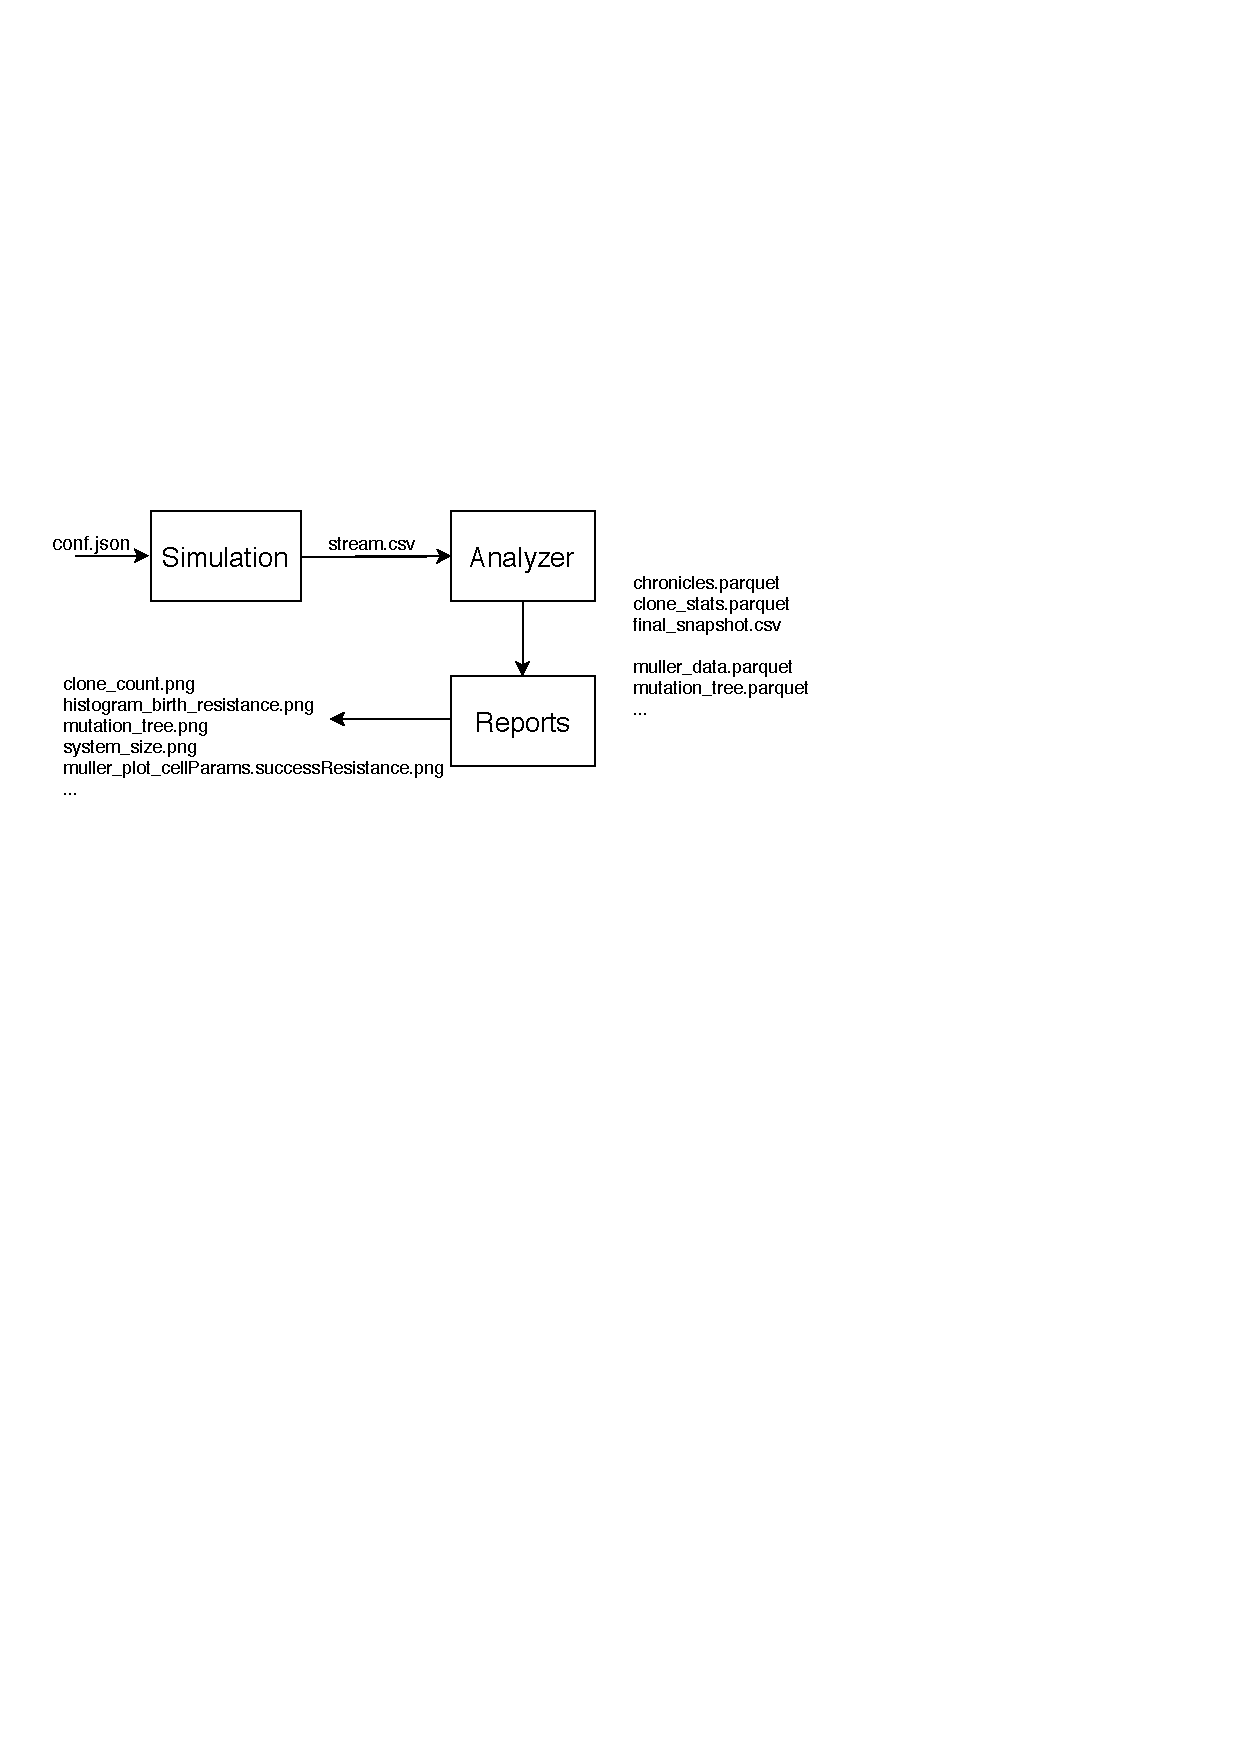
\includegraphics[width=0.9\linewidth]{diagrams/simbad-data-flow.pdf}
	\caption{Data flow between system components}
	\label{fig:data-flow}
\end{figure}

Each step has many dependencies on external libraries that need to be installed on host system and many configuration options that need to be set in order to execute the step. Due to high complexity of system, substantial amount of technical knowledge is needed to run the simulation process, and non-technical user are effectively unable to use this system, without help and guidance of its authors. Moreover, even if the user has required knowledge and skills to install and configure the system, system dependency on third-party code libraries that are not compatible with user machine may prevent the usage of the system.

To enable to users to use this system, an ease to use interface that will allow to control and monitor SimBad simulation process, and ability to install the system in host agnostic way are needed. The purpose of this thesis is to propose and implement such interface. 
Apart of ease of use, several other assumptions were made:
\begin{itemize}
    \item additional system components will be build on top of existing components without modifying them
    \item minimizing the resource footprint on host system
    \item host-agnostic installation
    \item decoupling of components
    \item zero-configuration needed for normal user and extensive configuration available to power user
\end{itemize}
In this thesis I will address each of those assumptions

% %\bibliographystyle{plalpha}
% \bibliographystyle{plabbrv}

% \bibliography{bibliography}
% \appendix
% \chapter{Configuration objects definitions}
\label{appendix:A}
Parameters that can be defined in simulation configuration file are defined in \textit{configurationSchema.json} file. Simulation files have tree structure and consist of several root objects that have multiple child objects, but for simplicity and re-usability, in schema those parameters are defined as flat list.

\begin{lstlisting}[label=list:param-def,caption=Parameter definitions in schema, basicstyle=\footnotesize\ttfamily]
[
    "paramName1": {...},
    "paramName2": {...}
]
\end{lstlisting}

The order in which parameters are defined in schema does not matter, as long as all parameters that other parameters depend on are defined. There are several parameter types
\section{Simple parameter}
This parameter type consists of single floating, integer or string value. It cannot have any child parameters. Example of such parameters in simulation file - \textit{sigma}, \textit{gamma} and \textit{scale} are simple parameters.
\begin{lstlisting}[label=list:simple-param,caption=Simple parameter definition, basicstyle=\footnotesize\ttfamily]
"parameters": {
    "sigma": "5",
    "gamma": "2",
    "scale": "10"
}
\end{lstlisting}
Definition for such parameter in `configurationSchema.json` looks like this:
\begin{lstlisting}[label=list:simple-param-def,caption=Simple parameter definition, basicstyle=\footnotesize\ttfamily]
"sigma": {
    "type": "simple",
    "description": "Some parameter description",
    "parameterType": "int",
    "minValue": 0,
    "maxValue": 1000,
    "defaultValue": 1
},
\end{lstlisting}

\section{Enum parameter}
Enum parameter is parameter that changes its child parameters based on its class - \textit{saturation} is an example of such parameter - it has two possible classes \textit{`inverse\_generalized\_exponential} and \textit{genralized\_exponential}

\begin{lstlisting}[label=list:enum-param-ex1,caption=Enum parameter example, basicstyle=\footnotesize\ttfamily]
"saturation": {
    "class": "inverse_generalized_exponential",
    "parameters": {
        "sigma": "10",
        "gamma": "2",
        "scale": "1000"
    }
},
\end{lstlisting}

Same parameter with different class would look like this:
\begin{lstlisting}[label=list:enum-param-ex2,caption=Enum parameter example, basicstyle=\footnotesize\ttfamily]
"saturation": {
    "class": "generalized_exponential",
    "parameters": {
        "sigma": "5",
        "gamma": "2",
        "scale": "10"
    }
}
\end{lstlisting}
Definition for such parameter in schema:
\begin{lstlisting}[label=list:enum-param-def,caption=Enum parameter definition, basicstyle=\footnotesize\ttfamily]
"saturation": {
    "type": "enum",
    "description": "Some description",
    "possibleClasses": [
        "generalized_exponential",
        "inverse_generalized_exponential"
    ],
    "defaultValue": "generalized_exponential"
}
\end{lstlisting}
\section{Complex}
Complex - this parameter type has one or more simple, complex or enum children. In example below \textit{generalized\_exponential} is such parameter - it has 3 simple children.
\begin{lstlisting}[label=list:complex-param-ex,caption=Complex parameter example, basicstyle=\footnotesize\ttfamily]
"saturation": {
    "class": "generalized_exponential",
    "parameters": {
        "sigma": "5",
        "gamma": "2",
        "scale": "10"
    }
},
\end{lstlisting}
\textit{Mutator} is an example of complex parameter with complex children :
\begin{lstlisting}[label=list:complex-ex,caption=Complex parameter example, basicstyle=\footnotesize\ttfamily]
"mutator": {
    "efficiency": {
        "class": "uniform_step",
        "parameters": {
            "increase_length": "0.1",
            "decrease_length": "1.0"
        }
    },
    "resistance": {
        "class": "uniform_step",
        "parameters": {
            "increase_length": "0.1",
            "decrease_length": "1.0"
        }
    }
}
\end{lstlisting}
Definition of such parameter is analogous to enum parameter, but instead of \textit{possibleClasses} that parameter can have, array of \textit{childClasses} is defined:
\begin{lstlisting}[label=list:complex-def,caption=Complex parameter definition, basicstyle=\footnotesize\ttfamily]
"mutator": {
    "type": "complex",
    "description": "Mutator description",
    "childClasses": ["efficiency", "resistance"]
},
\end{lstlisting}
% \chapter{Installation instruction}
\section{Windows}
\begin{enumerate}
    \item Install Docker for Windows using instructions from: \newline
    https://docs.docker.com/docker-for-windows/install/
    \item Enable hyper-v using instructions from: \newline
    https://docs.docker.com/docker-for-windows/install/
    \item Restart the computer
    \item Click Docker icon in tray and enable option "Switch to Linux Containers..." \newline
        \begin{minipage}{\linewidth}
            \centering
        	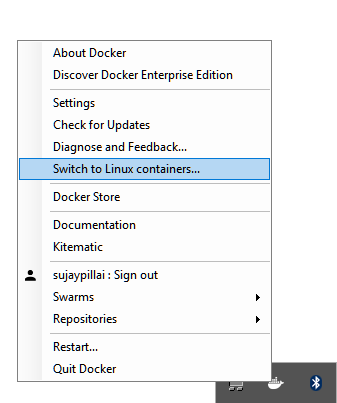
\includegraphics[width=0.4\linewidth]{instructions/systemtray.png}
        \end{minipage}
    \item Optional - open docker settings by clicking settings option and  in adavanced settings adjust how much resources can docker containers use
        \begin{minipage}{\linewidth}
            \centering
        	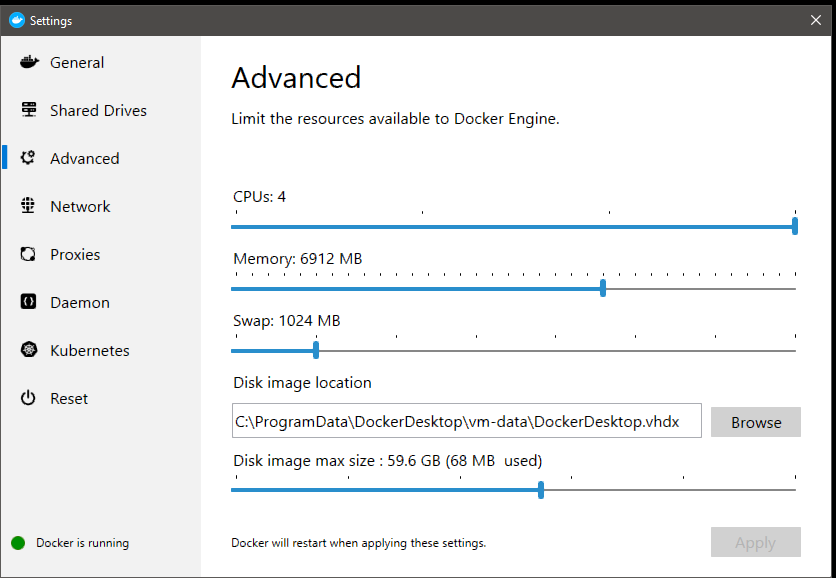
\includegraphics[width=0.4\linewidth]{instructions/res.PNG}
        \end{minipage}
    \item Clone or download repository from: \newline
     https://github.com/JakubSokolowski/simbad-monorepo
    \item Open powershell by pressing windows+R, typing "powershell" and pressing enter.
    \item From inside of powershell change directory to directory when the cloned repository is. The easiest way to do that is to find folder containing repository in Windows Explorer, type "cd " in powershell and drag and drop this folder onto powershell window. The command in powershell should now look like "cd C:\textbackslash Users \textbackslash Alice \textbackslash simbad\-monorepo". Press enter to execute it.
    \item While in cloned folder, enter command docker-compose -f docker/prod-docker-compose.yml up. This will start the download process - this operation may take around 15 mins depending on the internet connection and will download around 4GB of data. \newline
        \begin{minipage}{\linewidth}
            \centering
        	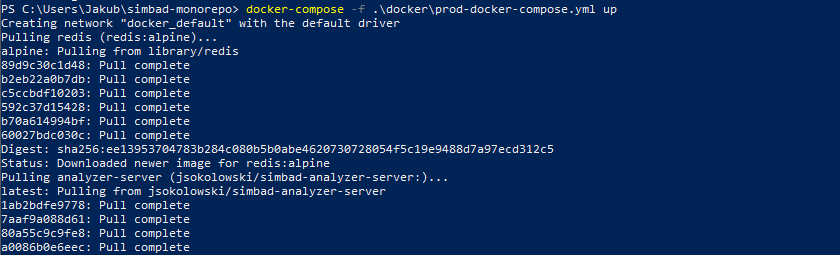
\includegraphics[width=0.9\linewidth]{instructions/docker2.PNG}
        \end{minipage}
    \item Docker will prompt you to enter password for, to grant access to host filesystem. Enter user password for each such prompt. \newline
    \begin{minipage}{\linewidth}
        \centering
        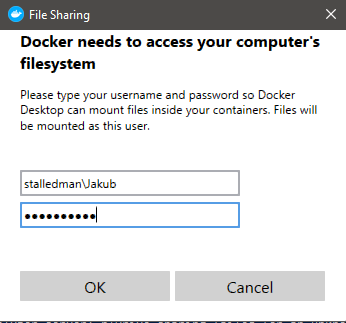
\includegraphics[width=0.5\linewidth]{instructions/docker3.PNG}
    \end{minipage}
    \item After command finishes executing, go to \textit{http://localhost:8080/\#/examples/simulation-pipeline } in browser.
    \item To stop, press ctrl+c in powershell
\end{enumerate}
\section{Linux}
\begin{enumerate}
    \item Install Docker using instructions from: \newline
    \textit{https://docs.docker.com/install/}
    \item Install Docker Compose using official instructions from: \newline
    \textit{https://docs.docker.com/compose/install/}
    \item Clone or download repository from: \newline
     https://github.com/JakubSokolowski/simbad-monorepo
    \item Open the terminal in the root folder of cloned repository
    \item Enter command docker-compose -f docker/prod-docker-compose.yml up. This will start the download process - this operation may take around 15 mins depending on the internet connection and will download around 4GB of data.
    \item Go to \textit{http://localhost:8080/\#/examples/simulation-pipeline } in browser
    \item To stop, press ctrl+c in terminal
\end{enumerate}

\chapterstyle{noNumbered}
\phantomsection % sets an anchor
\addcontentsline{toc}{chapter}{Indeks rzeczowy}
\printindex

\end{document}
